\section{Arquiteturas Paralelas}\label{sec:arquitetura}

Algumas das primeiras perguntas a serem feitas em relação ao desenvolvimento de aplicações é: por que estudar programação paralela?, os programas já não são rápidos o suficiente? as máquinas já não são rápidas o suficiente? Um dos principais pontos de motivação é que os requisitos necessários estão sempre mudando. Os usuários desejam executar aplicações e jogos cada vez mais detalhistas e com tempo de resposta menor. Além de que, desde 2005, é difícil encontrar um processador de um só \textit{core} no mercado~\cite{fruehe2005multicore, gepner2006multi}.

Outros motivos para utilizar programação paralela são: (i) reduzir o tempo necessário para solucionar um problema e (ii) resolver problemas mais complexos e de maior dimensão em um tempo aceitável. Existem além desses, outros motivos como: utilizar recursos computacionais subaproveitados; ultrapassar limitações de memória quando a memória disponível num único computador é insuficiente para a resolução do problema; e também ultrapassar os limites físicos que atualmente começam a restringir a possibilidade de construção de computadores sequenciais cada vez mais rápidos.

Nesse sentido, a computação de alto desempenho tem sido responsável por uma revolução científica. A evolução das arquiteturas de computadores melhorou o poder computacional, aumentando a gama de problemas e a qualidade das soluções que poderiam ser resolvidas no tempo requerido como, por exemplo, a previsão do tempo. Entretanto, devido a limitações de consumo de energia, dissipação de calor, dimensão do processador e uma melhor distribuição das \textit{threads} para processamento, a indústria mudou seu foco para arquiteturas paralelas e sistemas distribuídas~\cite{hsu2015three,borkar2011future,coteus2011technologies}.

A principal característica dessas arquiteturas é a presença de vários núcleos de processamento operando simultaneamente. No entanto, o desenvolvimento de \textit{software} foi afetado por essa mudança de paradigma e diversas aplicações sofreram reengenharias para tornar possível o aproveitamento dos recursos através da execução paralela~\cite{Gropp2013,Mittal2015,Cruz2016}.

\subsection{Classificação de Arquiteturas Paralelas}

A classificação de Flynn~\cite{flynn1996parallel} baseia-se no fato de um computador executar uma sequência de instruções sobre uma sequência de dados. As instruções e os dados são separados em um ou vários fluxos de instruções (\textit{instruction stream}) e um ou vários fluxos de dados (\textit{data stream}). Essa classificação possui quatro classes, mas vamos nos concentrar apenas nas duas classes que representam as arquiteturas paralelas: \textit{Single Instruction Multiple Data} (SIMD) e \textit{Multiple Instruction Multiple Data} (MIMD). A Figura~\ref{fig:simd_mimd} apresenta os diagramas das classes exemplificadas a seguir.

\begin{figure}[!htb]
	\centering
	\caption{Diagramas das classes SIMD (esquerda) e MIMD (direita).}
	\label{fig:simd_mimd}
	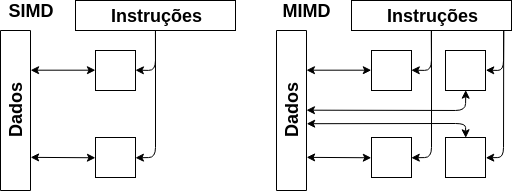
\includegraphics[scale=0.6]{flynn.png}
\end{figure}

Em uma arquitetura SIMD, uma única instrução é executada ao mesmo tempo sobre múltiplos dados. Esse processamento é controlado por uma única unidade de controle que é alimentada por um único fluxo de instruções. Cada instrução é enviada para todos processadores que executam as instruções em paralelo de forma síncrona sobre diferentes fluxos de dados. Essa arquitetura é encontrada nas unidades MMX/SSE de processadores \textit{multicore} e nas \textit{Graphics Processing Units} (GPUs).

Em arquiteturas MIMD, cada unidade de controle recebe um fluxo de instruções próprio e repassa-o para seu respectivo processador. Dessa forma, cada processador executa suas instruções em seus dados de forma assíncrona. O princípio dessa classe é bastante genérico, pois se um computador de um grupo de máquinas for analisado separadamente, este pode ser considerado uma máquina MIMD. Nessa classe encontram-se as arquiteturas paralelas \textit{multicore}.

Arquiteturas paralelas atuais combinam ambas arquiteturas SIMD e MIMD. Por exemplo, um processador \textit{multicore} possui vários \textit{cores} cada um trabalhando sobre um conjunto de instruções e um conjunto de dados, ou seja, MIMD. Em cada \textit{core} do mesmo processador existe uma unidade especial de ponto flutuante que explora SIMD. Sistemas distribuídos são compostos por várias arquiteturas paralelas, logo, combinando SIMD e MIMD.

\subsection{Arquiteturas Multicore e Manycore}

Desde 2003, a indústria vem seguindo duas abordagens para o projeto de microprocessadores~\cite{kirk2016programming}. A abordagem multicore é orientada à latência, onde instruções são executadas em poucos ciclos de \textit{clock}. Por outro lado, as arquiteturas manycore tem uma abordagem focada ao \textit{throughput}, ou seja, um grande número de instruções é executado por unidade de tempo.

O projeto das arquiteturas multicore e manycore é diferente ao ponto que dependendo da aplicação, o desempenho pode ser muito grande em uma arquitetura e muito pequeno na outra~\cite{cook2012cuda}. A arquitetura multicore utiliza uma lógica de controle sofisticada para permitir que instruções de uma única \textit{thread} sejam executadas em paralelo. Grandes memórias \textit{cache} são fornecidas para reduzir latências de acesso às instruções e dados de aplicações que tem acesso à memória predominante. Por fim, as operações das Unidades Lógicas e Aritméticas (ULA) também são projetadas visando otimizar a latência.

A arquitetura manycore tira proveito de um grande número de \textit{threads} de execução. Pequenas memórias \textit{cache} são fornecidas para evitar que múltiplas \textit{threads}, acessando os mesmos dados, precisem ir até a memória principal. Além disso, a maior parte do \textit{chip} é dedicada a unidades de ponto flutuante. Arquiteturas desse tipo são projetadas como mecanismos de cálculo de ponto flutuante e não para operações convencionais, que são realizadas por arquiteturas multicore. Algumas aplicações poderão utilizar tanto multicore quanto manycore em conjunto, sendo cada arquitetura melhor para um tipo de operação.